\documentclass[article]{jss}\usepackage{knitr}

%% -- LaTeX packages and custom commands ---------------------------------------

%% recommended packages
\usepackage{thumbpdf,lmodern}
\usepackage{float,tikz}
%% another package (only for this demo article)
\usepackage{framed}
%% author pakckage
\usepackage{xcolor,caption, float}

\graphicspath{ {./imgs/} }

%% new custom commands
\newcommand{\class}[1]{`\code{#1}'}
\newcommand{\fct}[1]{\code{#1()}}



%% -- Article metainformation (author, title, ...) -----------------------------

%% - \author{} with primary affiliation
%% - \Plainauthor{} without affiliations
%% - Separate authors by \And or \AND (in \author) or by comma (in \Plainauthor).
%% - \AND starts a new line, \And does not.
\author{Thomas Huet\\UMR 5140}
%   \And Second Author\\Plus Affiliation}
\Plainauthor{Thomas Huet}

%% - \title{} in title case
%% - \Plaintitle{} without LaTeX markup (if any)
%% - \Shorttitle{} with LaTeX markup (if any), used as running title
\title{Modelling Prehistorical Iconographic Compositions. The \proglang{R} package \pkg{decorr}}
\Plaintitle{Modelling Prehistorical Iconographic Compositions. The R package 'decorr'}
\Shorttitle{Modelling Prehistorical Iconographic Compositions}

%% - \Abstract{} almost as usual
\Abstract{
  By definition, Prehistorical societies are characterised by the absence of a writing system. During, the largest part of human history -- from far -- symbolic expressions belong to illiterate societies which express themself with rock-art paintings, pottery decorations, figurines and statuary, etc., and a lot of now disappeared carved woods, textil design, etc. At the composition level, recognition of meaningful associations of signs and reccurent patterns indicate clearly the existence of social conventions in the way to display and to read these expressions.
  We present the \pkg{decorr} \proglang{R} package which grounds concepts, methods and tools to analyse any ancient graphical systems. Our asumption is that i) any graphical system is a spatial distribution of features, and ii) these features have possibly any meaningful relationships one with another depending on their pairwise spatial proximities. To model the graphical compositions we employ concepts coming from the Graph Theory. To ensure the feasability of this type of analysis, we propose a GIS-based method for inputs and a serie of functions for data management.   
}

\Keywords{Iconography, Prehistory, Graph Theory, Graph Drawing, Spatial Analysis, \proglang{R}}
\Plainkeywords{Iconography, Prehistory, Graph Theory, Graph Drawing, Spatial Analysis, R}

\Address{
  Thomas Huet\\
  CNRS-UMR 5140 \\
  Archeologie des Societes Mediterraneennes\\
  Universite Paul Valery\\
  route de Mende\\
  Montpellier 34199, France\\
  E-mail: \email{thomashuet7@gmail.com}\\
%  URL: \url{https://eeecon.uibk.ac.at/~zeileis/}
}
\IfFileExists{upquote.sty}{\usepackage{upquote}}{}
\begin{document}
% \SweaveOpts{concordance=TRUE}
% \Sweave2knitr("article_rvTH14_1.Rnw")
% \SweaveOpts{concordance=TRUE}

\section[Introduction]{Introduction} \label{sec:intro}

Symbolic practices is a characteristic trait of human societies. Even discussed, such practices seems to start between 233,000 to 800,00 BC \citep{dErrico00}, covering more than 97\% of total human societies time span. Symbolism cover a large range of practices, from ochre deposit in a tomb, to menhir alignements, passing through wall fresco. This latter, what might be called "iconographical practices", probably shows the most complex and interesting testimonies of past societies symbolism. For decades, its study was linked to history of religion because commonly seen as closely linked to cultual practices and believes. Since the \textit{New Archaeology} developpement during the 60's \citep{Clarke14}, symbolic expressions start to be studied with the same formal methods (statistics, seriations, distribution maps, etc.) as any another aspect of social organisation: settlement patterns, tools \emph{chaine op\'eratoire}, susbsitence strategies, etc. \citep{Renfrew91}. But unlike many aspects of the material culture where technological requirements and technical efficiency determine the choice of the raw material and the of the object -- a flint blade for cutting, a pottery for containing, a house for living --, the function of an iconographic composition cannot be drawn directly from itself. Whether these last decades study of ancient iconography had  undergone significative improvements at the site scale -- with GIS/database statistics, paleoenvironmental restitutions, etc. -- and at the sign scale with the development of archaeological sciences -- radiocarbon dating, use-wear analysis, elemental analysis, etc. --, these improvement do not necessarly help to understand the semantic content of the iconography.

Semantics or semiotics can be defined as a system of conventional features -- called signs -- organised also in conventional manners. Until our days, formal methods to study ancient iconography semantics have been mostlty been grounded  -- explicitly or not -- on the prime principle of Saussurian linguistic: the '\emph{linearity of the signifier}' \citep{Saussure89}.  
Writing is one of the most rational semiographical system with a clear distinction between signified and signifier and the development of the signified on a linear axis. Even if we do not understand the meaning of the signs, writing can easily be modelled with Graph theory and recurent patterns can be identified. For example, the 3-letters word "\code{art}" can be modelled with three vertices (\code{a}, \code{r}, \code{t}) and two edges (one between \code{a} and \code{r}, the other between \code{r} and \code{t}). In \proglang{R}, these features, concatenated in this order with a \code{paste0()}, is \code{art}, and not \code{rat}.

\begin{figure}[H]

{\centering 
\includegraphics[width=\maxwidth]{figure/unnamed-chunk-1-1} 

}

\caption{\label{fig:figs}concatenate of graphical units (GUs) is art}\label{fig:unnamed-chunk-1}
\end{figure}



But, as stated, in Prehistorical the writing system does not exists. Spatial relationships between graphical features, or graphical units, are not necessarly linear and directed but could most probably be more multi-directional and undirected: the direction of the interactions of pairwise GUs can be in any order.

\begin{figure}[H]

{\centering 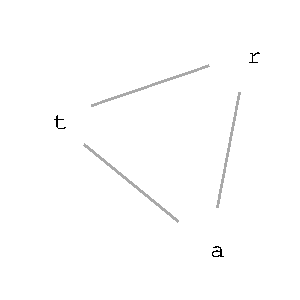
\includegraphics[width=\maxwidth]{figure/unnamed-chunk-2-1} 

}

\caption{\label{fig:figs}Potential spatial relations between GUs.}\label{fig:unnamed-chunk-2}
\end{figure}



Because of the inherent variability of iconography, and because graphical and spatial proximities between GUs are generaly not quantified, applying the Saussurian model to any prehistorical graphical content had led to considerable problems:
\begin{itemize}
\setlength\itemsep{.05em}
  \item unexplicit groupings of graphical units -- like graphical units grouped into \emp{figures},  \emp{figures} grouped into \emp{patterns}, \emp{patterns} grouped into \emp{motives}, etc. -- with tedious number of groups
  \item consistency, proximities and relationships between these groups are often implicit and not quantified
  \item studies develop proper descriptive vocabularies, singular relationships of grouped, idosyncratic methods in a site-dependend or period-dependend scales 
\end{itemize}

These issues limit drastically the possibility to conduct cross-cultural comparisons and to draw a synthesis of humankind's symbolism at a large scale and over the long-term. 
\\
\\
In this article we present the \proglang{R} package \pkg{decorr}. Its purpose is to formalise a method based on relative neighborhood graphs to analyse any graphical content. As any formal system, iconography can be modelled as spatial features related one with the other depending on rules of spatial proximities, as state by the First Law of Geography: "\emph{everything is related to everything else, but near things are more related than distant things}" \citep{Tobler70}. The principal idea of our model is that any graphical system can be represented by features connected (or not) to each other depending on their spatial proximity. To map and analyse these proximities, the model uses concepts and methods coming from Graph Theory. This package has been grounded on the seminal work of \citet{Alexander08} and its first IT implementation by \citet{Huet18a}. 

\section[Model]{Graph theory Model} \label{sec:model}

Graph theory offers a conceptual framework and indices (global at the entire graph scale, local at the vertex scale) to deal with notions of networks, relationships and neighbourhoods. Graphical units (GUs) can be modelled as vertices (nodes) and their spatial relations can be modelled as edges. The different levels of GUs spatial organisation can be retrieve by a relative neighborhood graphs analysis (Graph Theory) and a spatial (GIS) analysis.

Nodes and edges -- repectively GUs and connexions between GUs -- are created on a GIS interface. Indeed, for large series of graphical decorations, GIS offers the most suitable and flexible interface to register all GUs and to get their coordinates. These \emph{x} and \emph{y} coordinates, measured in pixels, are relative to the decoration figure which is open in the first place in a new GIS project without any projection system. The decoration image is considerated as the basemap of the project and will cover the region of interest of the analysis. The decoration image can be binarized: GUs are considerated active, the undecorated parts of the support -- the background -- are considerated inactive. The entire decoration image is tiled into different GUs' area of influence like a Voronoi diagram of the support where the Voronoi seeds are the GUs. Exist a link between a pair of GUs when their area of influence share a common border. A RNG -- also called a geometric graph, or a planar graph -- is constructed from GUs (nodes) and their proximity links (edges). The graph itself is as a subgraph of a Delaunay triangulation.


\begin{figure}[H]
\centering
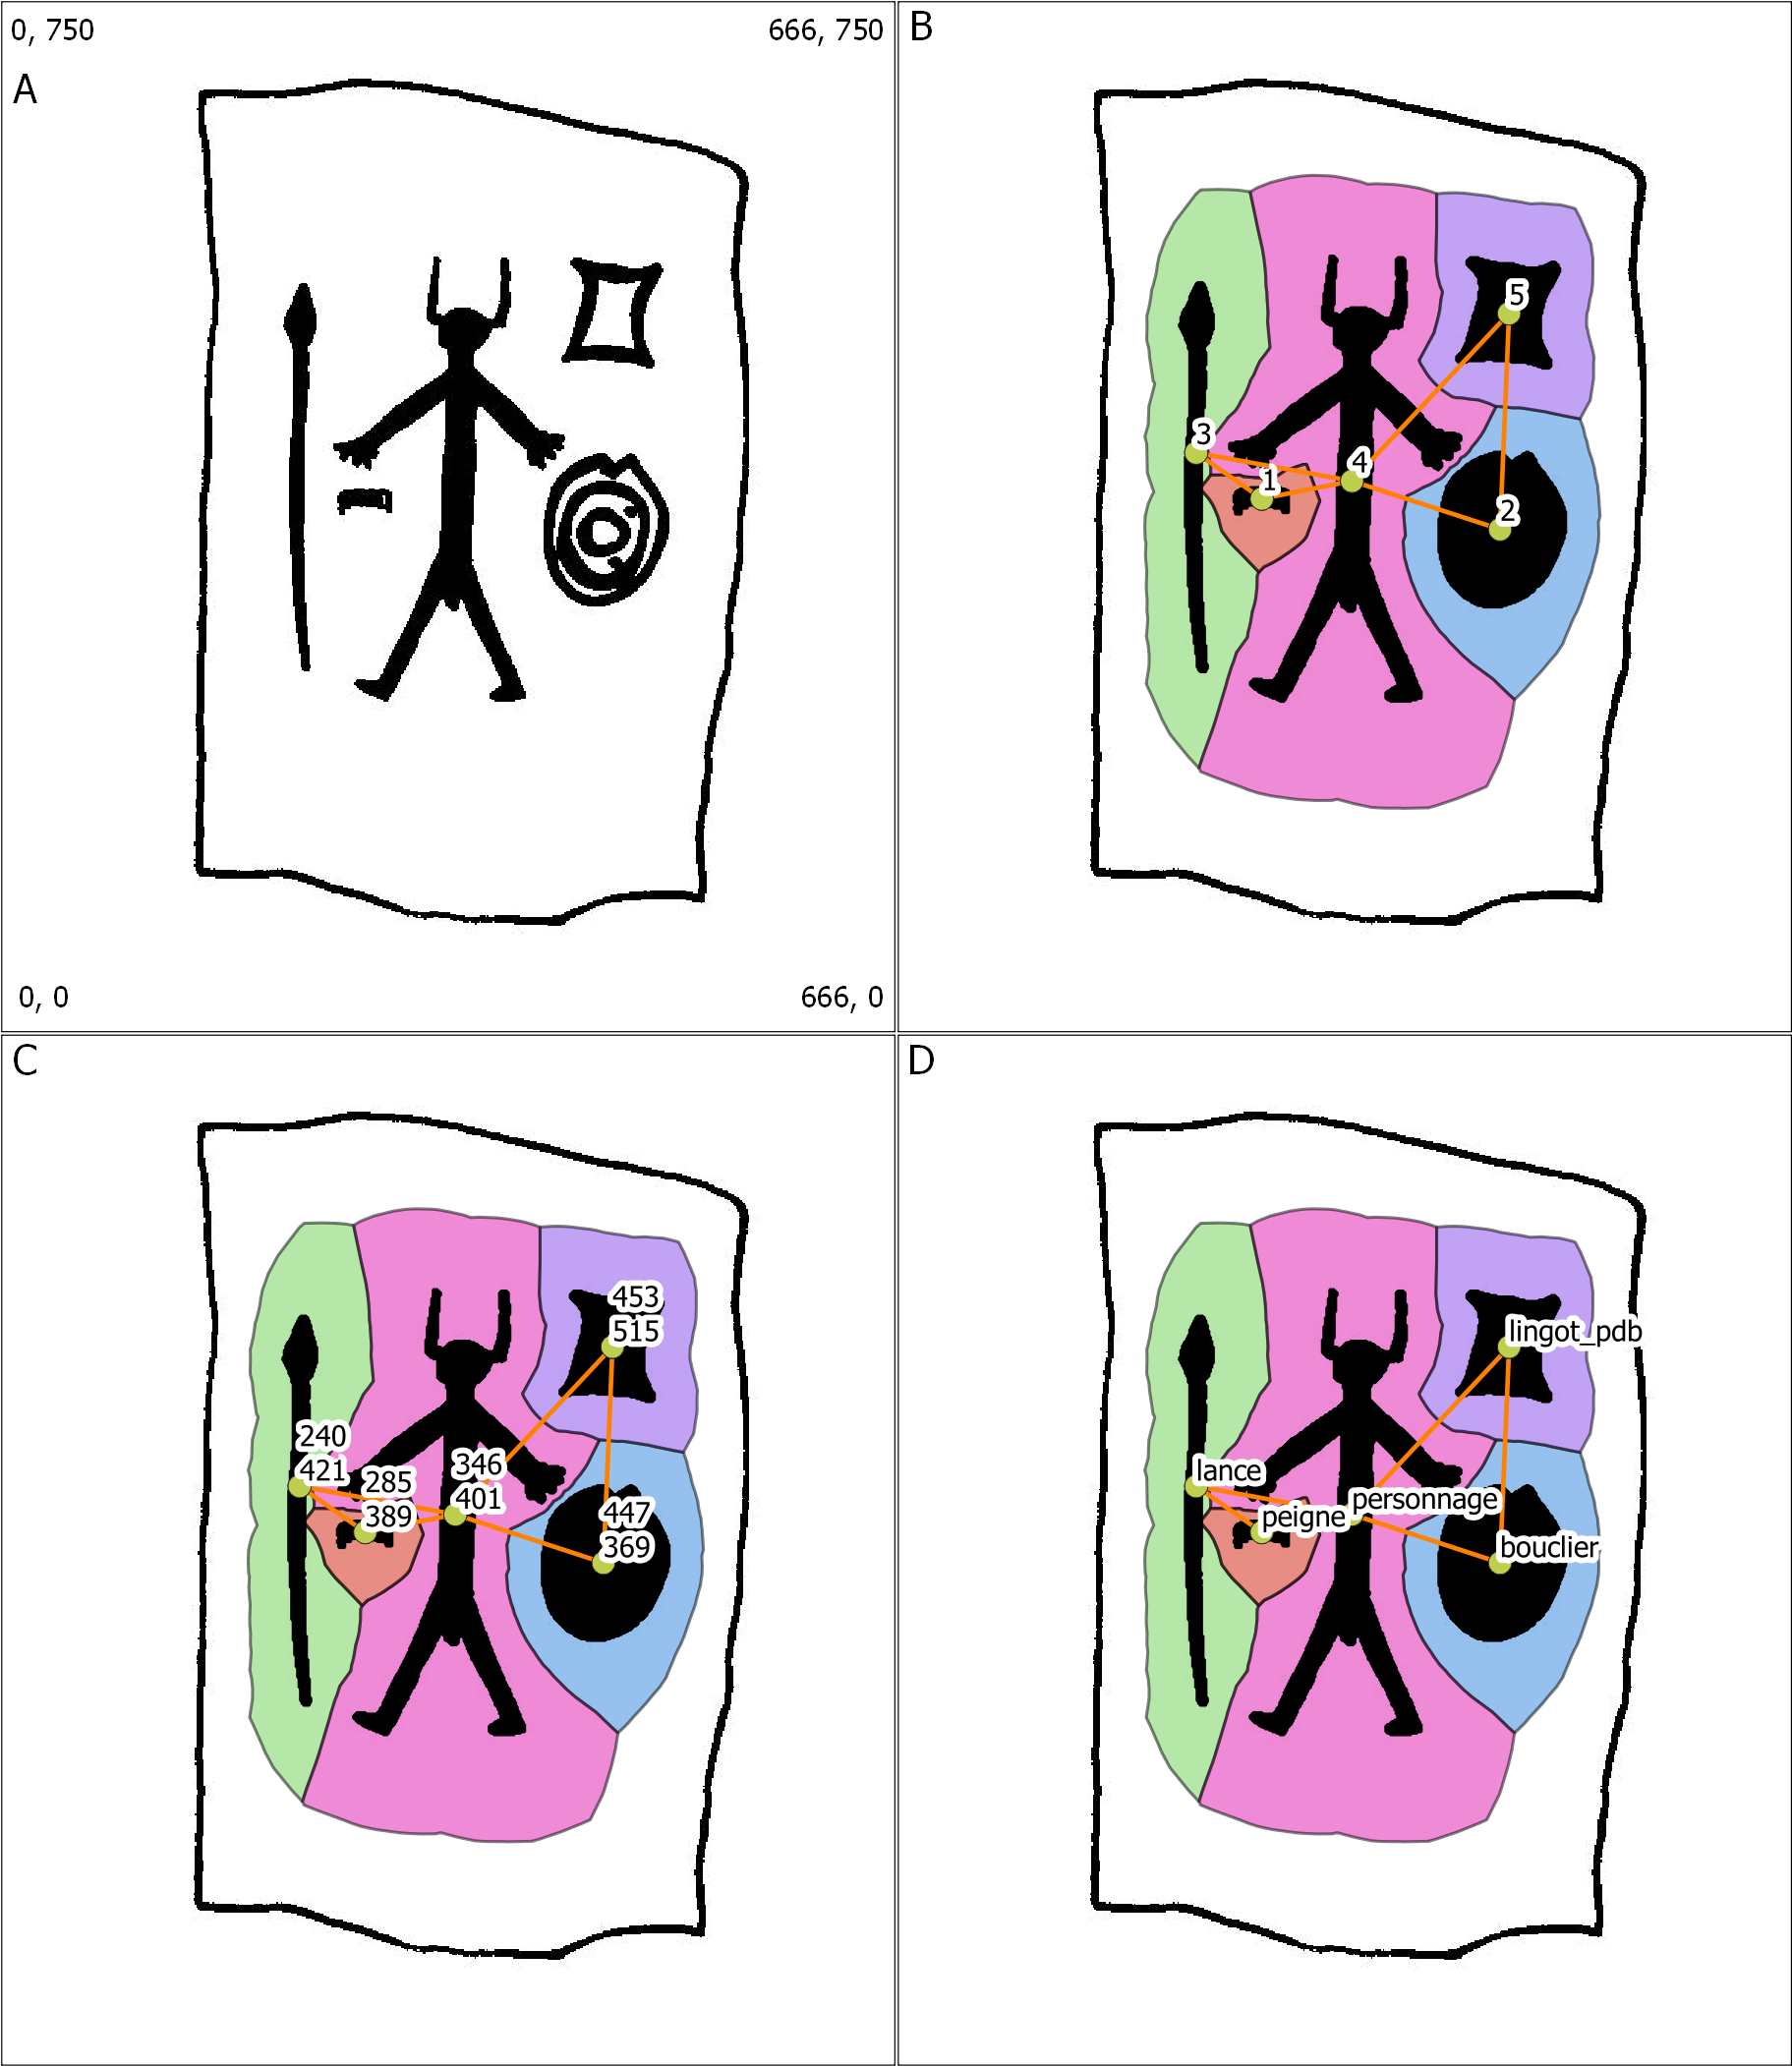
\includegraphics{gis}
\caption{\label{fig:gis} GIS interface. A) Original decoration of the Late Bronze Age \emp{Cerro Muriano 1} stele (drawing: \cite{DiazGuardamino10}) with its extent (\code{xmin, xmax, ymin, ymax}); B) After the polygonisation of the GUs, including the border of the stelae, the Voronoi cells, the centroid of GUs and the links between GUs having adjacent cells (ie, sharing a border) are calculated; C) For each GUs, \emph{x} and \emph{y} are calculated; D) At least one variable, like the \code{type} of the GUs is defined in order to compute composition analysis. A simplier solution will be to create directly centroids (\code{POINTS}) on the GUs and to draw the edges manually}
\end{figure}

This model has a minimal of \emph{a priori} definitions. Those definitions only concern the intrinsic properties of GUs (type, technology, color, orientation, size, etc.) and the types of relations they share. Here, we will only consider one property for the nodes, its type (column \code{type}), and the most common types of relations between GUs: \emph{normal}, \emph{attribute} and \emph{overlapping} edges.

\begin{itemize}
  \item \emph{normal} edges
\end{itemize}

By convention, two different GUs having a Voronoi cell sharing a border, have a common edge tagged \code{'='} and represented with a plain line. The textual notation of such an edge is \code{'-=-'}. For example: \code{1 -=- 4} means that the nodes \code{1} and \code{4} have a common border.

\begin{itemize}
  \item \emph{attribute} edges
\end{itemize}

It occurs frequently that a GU can be divided into a \emph{main unit} (eg, a character) and one or various \emph{attribute units} (eg, a helmet, male sex). Broadly speaking, for further statistical analysis, it is better to use this \emph{attribute} method than to multiply the categories of GUs. To record this information, a new type of edge, tagged with \code{'+'}, is be introduced. This type of edges is directed and, by convention, displayed with a dashed line. Its starts from the \emph{main unit} and ends with the \emph{attribute units}. The textual notation of such an edge is \code{'-+-'}. For example \code{4 -+- 6} means that the main node \code{4} has the attribute node \code{6}.

\begin{figure}[H] 
\centering
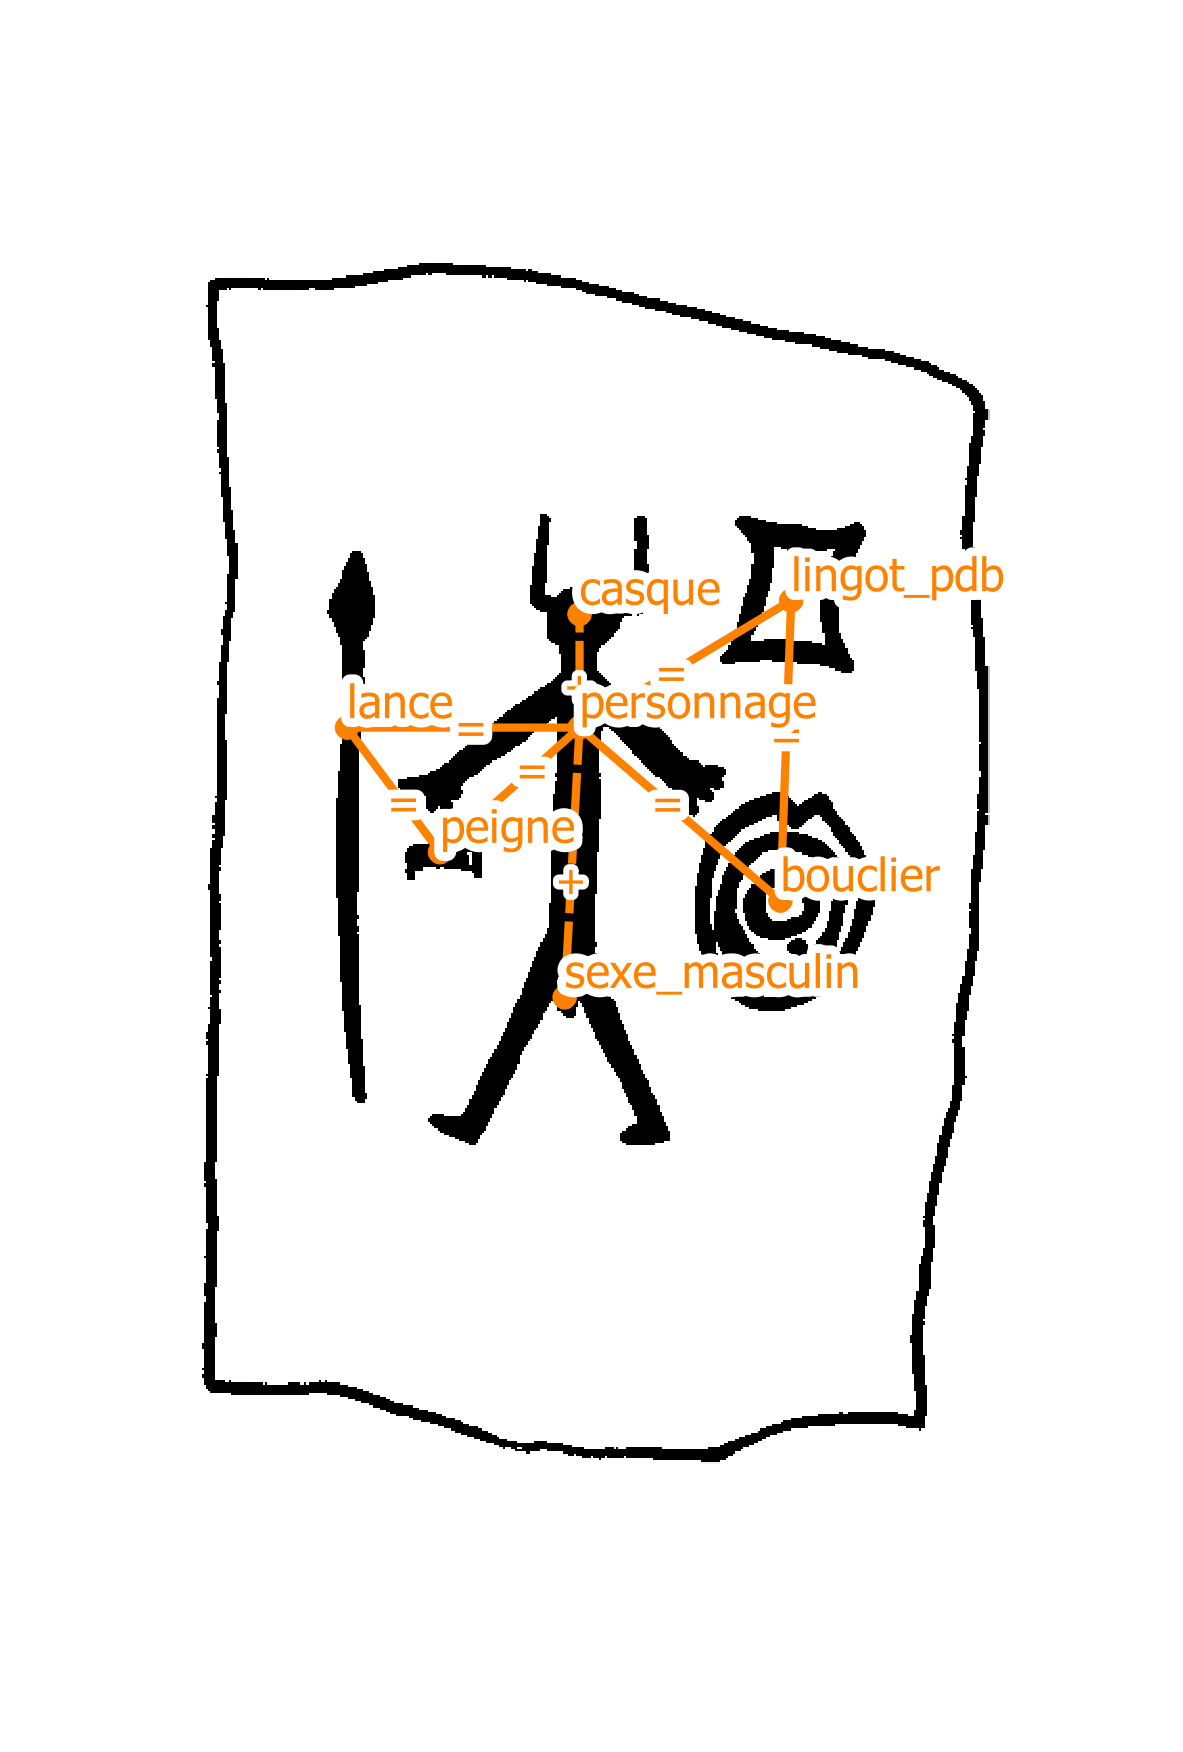
\includegraphics[scale=0.15]{gis_1}
\caption{\label{fig:gis1} GIS interface. The GUs \code{casque} (helmet) and \code{sexe\_masculin} (male sex) are two attributes of the GU \code{personnage} (character).}
\end{figure}

\begin{itemize}
  \item \emph{overlapping} edges
\end{itemize}

Finally, it is quite common that a graphical composition shows superimpositions between different UGs permit to distinguish different decoration phases for a single support. So, at first, the analyse must be performed on each different phases of decoration separately. This stratigraphical information (\code{A} \emph{over} \code{B}, or \code{B} \emph{under} \code{A}) helps to understand the relative chronology between GUs and must be recorded. A simple way to achieve this is to introduce the new tag \code{'>'} for the for the type of edge. This type of edges is directed. The textual notation of such an edge is \code{'->-'}. For example \code{A ->- B} means that \code{A} crosses \code{B} (ie, \code{A} overlaps \code{B} in the stratigraphical sense).

\section{The R package decorr} \label{sec:models}

The \pkg{decorr} package can be downloaded from GitHub
%
\begin{CodeChunk}
\begin{CodeInput}
R>   devtools::install_github("zoometh/iconr", build_vignettes=TRUE)
\end{CodeInput}
\end{CodeChunk}
%

\subsection{External package} \label{sec:ext_pck}

The \pkg{decorr} package imports the following packages:
\begin{itemize}
\setlength\itemsep{.1em}
  \item \pkg{magick} for image manipulation \citep{Ooms18}
  \item \pkg{igraph} for graph and network analysis \citep{Csardi06} 
  \item \pkg{rgdal}  to read \emph{shapefiles} of nodes and edges \citep{Bivand19}
  \item \pkg{grDevices} for colors and font plotting, \pkg{graphics} for graphics, \pkg{utils} and \pkg{methods} for formally defined methods and \emph{varia} methods (all combinations, etc.) \citep{R19}
\end{itemize}

\subsection{Data} \label{sec:ext_data}

A training dataset (nodes and edges coordinates, decoration images) is stored in the \code{extdata} folder of the \pkg{decorr} package

\begin{itemize}
\item The \code{imgs} dataframe
\end{itemize}

The dataframe storing the inventory of decorations is \code{imgs}. The field \code{imgs$idf} is the short name of the decoration, useful during statistical analysis. The primary key of each decoration is the concatenate of \code{imgs$site} and \code{imgs$decor}. These keys will allow joints with the other dataframes (\code{nodes} and \code{edges})\\
%
% latex table generated in R 3.6.1 by xtable 1.8-4 package
% Tue Nov 03 09:11:03 2020
\begin{table}[H]
\centering
\begin{tabular}{|p{0.5cm}|p{2.5cm}|p{2.5cm}|p{8.5cm}|}
  \hline
idf & site & decor & img \\ 
  \hline
  1 & Cerro Muriano & Cerro Muriano 1 & Cerro\_Muriano.Cerro\_Muriano\_1.jpg \\ 
    2 & Torrejon Rubio & Torrejon Rubio 1 & Torrejon\_Rubio.Torrejon\_Rubio\_1.jpg \\ 
    3 & Brozas & Brozas & Brozas.Brozas.jpg \\ 
    4 & Zarza de Montanchez & Zarza De Montanchez & Zarza\_de\_Montanchez.Zarza\_De\_Montanchez.jpg \\ 
   \hline
\end{tabular}
\caption{The studied corpus, the \code{imgs.tsv} dataframe} 
\label{Test_table}
\end{table}

%
The \pkg{decorr} package training dataset is composed by four stelaes decorations drawings \citep{DiazGuardamino10} belonging to the so-called 'Warrior stelae' family -- with about 140 stelae -- dated to the Late Bronze Age of SW Iberian peninsula \citep{Celestino01}. At first the drawings dataset can be checked by using the \code{imgs} dataframe and the \pkg{magick} package.
%
\begin{kframe}
\begin{verbatim}
R> library("magick")
R> pth <- system.file("extdata", package = "decorr")
R> imgs <- read.table(system.file("extdata", "imgs.tsv", package = "decorr"),
+                     sep="\t", stringsAsFactors = FALSE)
R> lims <- list()
R> for(i in 1:nrow(imgs)){
+    i1 <- image_read(paste0(pth,"\\",imgs[i,"img"]))
+    lbl.txt <- paste0(imgs[i,"idf"],"\n",
+                      imgs[i,"site"],"\n",
+                      imgs[i,"decor"],"\n",
+                      imgs[i,"img"],"\n",
+                      image_info(i1)$width,"*",image_info(i1)$height," px")
+    i1 <- image_annotate(i1,lbl.txt,location = "northwest",
+                         size = 25, color = "red")
+    lims[[length(lims)+1]]<- i1
+  }
R> out.img <- image_append(c(image_append(c(lims[[1]],lims[[2]])),
+                            image_append(c(lims[[3]],lims[[4]]))),
+                          stack = TRUE)
R> plot(out.img)
\end{verbatim}
\end{kframe}\begin{figure}[H]

{\centering 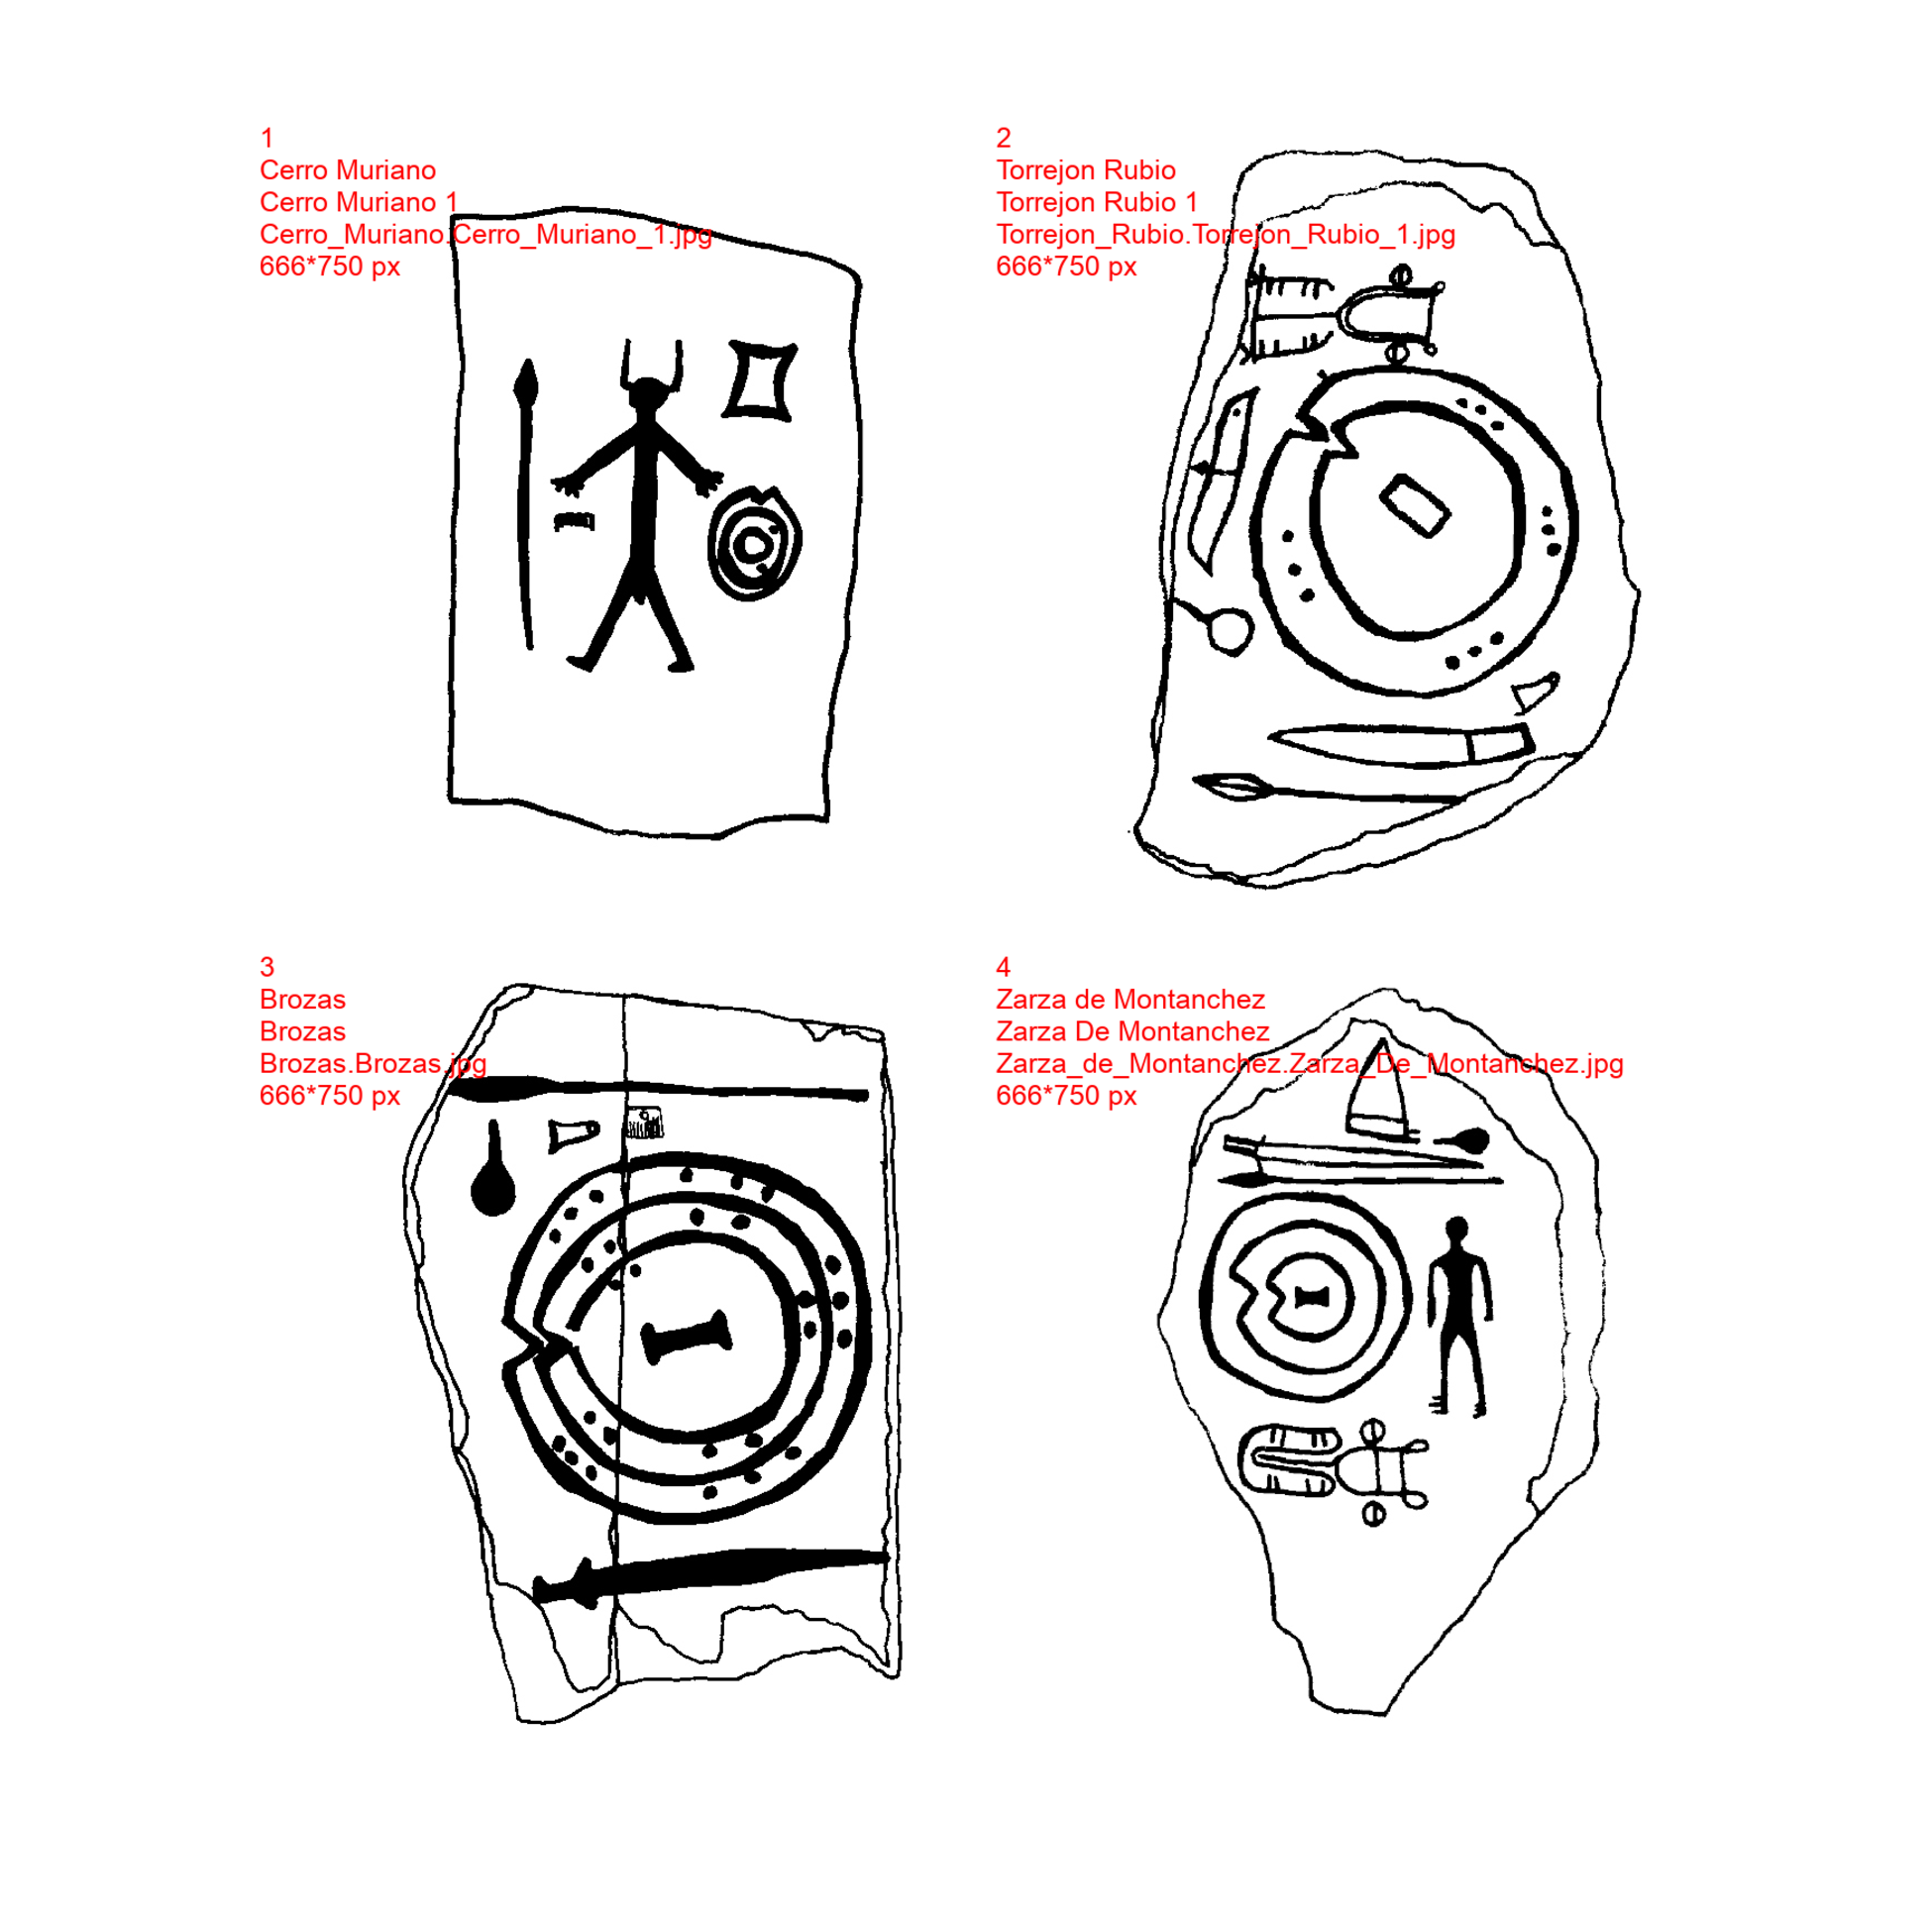
\includegraphics[width=\maxwidth]{figure/unnamed-chunk-4-1} 

}

\caption{\label{fig:figs}Decoration images of the training dataset}\label{fig:unnamed-chunk-4}
\end{figure}


%
To construct a graph overlapping the decoration images listed in the \code{images} dataframe, the first step is to load \code{nodes} and \code{edges} dataframes.
%
\begin{kframe}
\begin{verbatim}
R> nodes <- read.table(system.file("extdata", "nodes.csv", package = "decorr"),
+                      sep=";",stringsAsFactors = FALSE)
R> edges <- read.table(system.file("extdata", "edges.csv", package = "decorr"),
+                      sep=";",stringsAsFactors = FALSE)
\end{verbatim}
\end{kframe}

\begin{itemize}
\item The \code{nodes} dataframe
\end{itemize}

It contains the required minimum variables for the analysis.

\begin{kframe}
\begin{verbatim}
R> caption <- "Nodes (from \\code{nodes.csv} dataframe)}"
R> print(xtable::xtable(head(nodes),
+                       caption = caption),
+        table.placement="H")
\end{verbatim}
\end{kframe}% latex table generated in R 3.6.1 by xtable 1.8-4 package
% Tue Nov 03 09:11:04 2020
\begin{table}[H]
\centering
\begin{tabular}{rllrlrr}
  \hline
 & site & decor & id & type & x & y \\ 
  \hline
1 & Cerro Muriano & Cerro Muriano 1 &   1 & personnage & 349.81 & -298.32 \\ 
  2 & Cerro Muriano & Cerro Muriano 1 &   2 & casque & 349.81 & -243.99 \\ 
  3 & Cerro Muriano & Cerro Muriano 1 &   3 & lance & 238.46 & -298.32 \\ 
  4 & Cerro Muriano & Cerro Muriano 1 &   4 & bouclier & 446.02 & -381.17 \\ 
  5 & Cerro Muriano & Cerro Muriano 1 &   5 & peigne & 283.00 & -358.01 \\ 
  6 & Cerro Muriano & Cerro Muriano 1 &   7 & sexe\_masculin & 342.69 & -427.49 \\ 
   \hline
\end{tabular}
\caption{Nodes (from \code{nodes.csv} dataframe)}} 
\end{table}


The primary key of the decoration is based on two fields: \code{nodes$site} and \code{nodes$decor}. The site is the current unit of analysis in Prehistory and Archaeology, but since a site can have various decorated objects, a primary key on two fields is necessary. The \code{nodes$id} is the identifier of the node. The \code{nodes$type} field is the default variable for further statistical analysis. Here, \code{nodes$type} refers to the typology of the GUs (anthropomorph, weapons, etc.). The \code{nodes$x} and \code{nodes$y} columns refer to the \emph{x} and \emph{}y coordinates of the nodes. As said, in the first place theses coordinates come from the GIS. But, in a GIS, the coordinates origin (0, 0) is the bottom-left corner and exist negative values, while this origin is top-left for any \proglang{R} matrices (rasters, grids, dataframes, etc.) with only positive values. To recover the correct the \emph{y} value of GUs nodes and edges, that is to say the \emph{y} value on the decoration image, the \pkg{decorr} calculate the absolute \emph{y} value and used the image height as a constant offset.

\begin{itemize}
\item The \code{edges} dataframe
\end{itemize}

The \code{edges} dataframe is quite similar to the \code{nodes} dataframe.

\begin{kframe}
\begin{verbatim}
R> caption <- "Edges (from \\code{edges.csv} dataframe)}"
R> print(xtable::xtable(head(edges),
+                 caption=caption,
+                 label="edgesdf"),
+        table.placement="H")
\end{verbatim}
\end{kframe}% latex table generated in R 3.6.1 by xtable 1.8-4 package
% Tue Nov 03 09:11:04 2020
\begin{table}[H]
\centering
\begin{tabular}{rllrrl}
  \hline
 & site & decor & a & b & type \\ 
  \hline
1 & Cerro Muriano & Cerro Muriano 1 &   1 &   8 & = \\ 
  2 & Cerro Muriano & Cerro Muriano 1 &   4 &   8 & = \\ 
  3 & Cerro Muriano & Cerro Muriano 1 &   1 &   4 & = \\ 
  4 & Cerro Muriano & Cerro Muriano 1 &   1 &   5 & = \\ 
  5 & Cerro Muriano & Cerro Muriano 1 &   3 &   5 & = \\ 
  6 & Cerro Muriano & Cerro Muriano 1 &   1 &   2 & + \\ 
   \hline
\end{tabular}
\caption{Edges (from \code{edges.csv} dataframe)}} 
\label{edgesdf}
\end{table}


Fields \code{edges$site} and \code{edges$decor} are the primary key of decoration. The fields \code{edges$a} and \code{edges$b} are the equivalent to columns \emph{from} and \emph{to} in Graph theory. Even if undirected graphs will the most common models in further studies, this direction helps to distinguish between nodes. The first column \code{edges$a} is the identifier of starting node or \emph{main node} or \emph{overlapping node}. The second column \code{edges$b} is the identifier of the ending node or \emph{attribue node} or \emph{overlapped node}. The \code{edges$type} is the type of relation (normal, attribute, overlapping, etc.) between the starting node and the ending node. There is no need to get the coordinates of the edges, these coordinates are calculated from the \code{nodes} dataframe. For example, Table \ref{edgesdf} shows that the first edge of the \emph{Cerro Muriano 1} decoration connects the nodes \code{1} and \code{8} (respectively in column \code{edges$a} and \code{edges$b}). A way to retrieve these connected nodes' coordinates will be:

\begin{kframe}
\begin{verbatim}
R> cm.1 <- subset(nodes, decor == "Cerro Muriano 1" & id == 1)[,c("x","y")]
R> cm.8 <- subset(nodes, decor == "Cerro Muriano 1" & id == 8)[,c("x","y")]
R> cat(as.numeric(cm.1),";",as.numeric(cm.8))
\end{verbatim}
\end{kframe}349.8148 -298.3244 ; 451.1489 -237.4782

Once these three dataframes loaded, the list of decoration graphs can be calculated with the \code{list_dec()} function.

\subsection{\code{list\_dec()} function} \label{sec:funlistdec}

The \code{list\_dec()} function allows to calculate graphs for all decorations stored into \code{nodes}, \code{edges} and \code{images}. The result is a list of decoration graph. The first graph of can be plotted

\begin{kframe}
\begin{verbatim}
R> par(mar=c(0.1,0.1,0.1,0.1))
R> library("decorr")
R> # imgs <- read.table(system.file("extdata", "imgs.tsv", package = "decorr"),
R> #                       sep="\t", stringsAsFactors = FALSE)
R> # nodes <- read.table(system.file("extdata", "nodes.csv", package = "decorr"),
R> #                     sep="\t",stringsAsFactors = FALSE)
R> # edges <- read.table(system.file("extdata", "edges.csv", package = "decorr"),
R> #                     sep="\t",stringsAsFactors = FALSE)
R> lgrph <- list_dec(imgs,nodes,edges,var="type")
R> plot(lgrph[[1]],
+       vertex.color = "orange",
+       vertex.frame.color="orange",
+       vertex.label.color = "black",
+       vertex.size = 8,
+       vertex.label.cex = 0.6,
+       edge.color = "orange",
+       vertex.label.family="Helvetica"
+  )
\end{verbatim}
\end{kframe}\begin{figure}[H]

{\centering 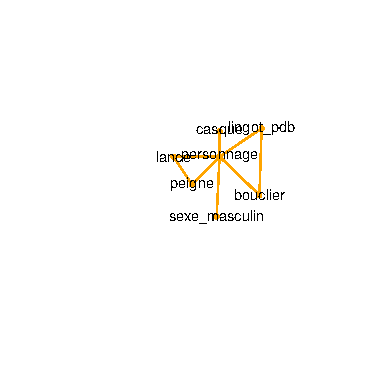
\includegraphics[width=\maxwidth]{figure/unnamed-chunk-8-1} 

}

\caption{\label{fig:figs}Plot of the first graph of the list}\label{fig:unnamed-chunk-8}
\end{figure}




The others \pkg{decorr} package functions can be divided into:
\begin{enumerate}
 \item graphical functions
 \item single decoration functions
 \item comparisons between different decorations functions
\end{enumerate}

\subsection{Graphical functions} \label{sec:functions_gr}

The \pkg{decorr} package has three graphical functions
\begin{itemize}
\setlength\itemsep{.1em}
\item \code{labels_shadow()} function is a re-use of the \code{shadowtext()} function from the \pkg{TeachingDemos} package \citep{Snow20}.
\item \code{side_plot_nds()} and \code{side_plot_eds()} allow to plot figures side-by-side for nodes or edges comparisons
\end{itemize}

\subsection{Single decoration functions} \label{sec:functions_one}

Functions allowing to create a RNG for a single decoration are:

\begin{itemize}
\setlength\itemsep{.1em}
  \item \code{read_nds()} and \code{read_eds()} functions allow to read respectively a file of nodes and a file of edges (\code{.tsv} or \code{.shp} files)
\end{itemize}

The \code{read_nds()} function is close to the \proglang{R} native \code{read.table()} function, but allows to read \emph{shapefiles} of nodes.

The \code{read_eds()} permits to read a \emph{shapefiles} of edges or to retrieve the coordinates of the the edges from the \code{nodes} dataframe. For example, the first \emph{Torrejon Rubio 1} edge, between the nodes \code{6} and \code{5}, has the starting point (xa = 366.7001, ya = -563.1358) and the ending point (xb = 490.1195, yb = -513.2428)

\begin{kframe}
\begin{verbatim}
R> # library(decorr)
R> sit <- "Torrejon Rubio" ; dec <- "Torrejon Rubio 1"
R> nds.df <- read_nds(site = sit, decor = dec, dev = ".tsv",
+                     doss = system.file("extdata", package = "decorr"))
R> eds.df <- read_eds(site = sit, decor = dec, dev = ".tsv",
+                     doss = system.file("extdata", package = "decorr"))
R> print(xtable::xtable(eds.df[1,],
+                       caption="first edge of the dataframe",
+                       label="Test_table_1",
+                       size=7),
+        table.placement="H")
\end{verbatim}
\end{kframe}% latex table generated in R 3.6.1 by xtable 1.8-4 package
% Tue Nov 03 09:11:04 2020
\begin{table}[H]
\centering
\begin{tabular}{rllrrlrrrr}
  \hline
 & site & decor & a & b & type & xa & ya & xb & yb \\ 
  \hline
9 & Torrejon Rubio & Torrejon Rubio 1 &   6 &   5 & = & 366.70 & -563.14 & 490.12 & -513.24 \\ 
   \hline
\end{tabular}
\caption{first edge of the dataframe} 
\label{Test_table_1}
\end{table}

\end{figure}

\begin{itemize}
\setlength\itemsep{.1em}
  \item \code{plot_dec_grph ()} allows to plot a RNG over a decoration image
\end{itemize}

Once, the \code{imgs}, \code{nodes} and \code{edges} dataframes have been read, the decoration graph is build and can be plotted, here for the \emph{Torrejon Rubio 1} decoration. The \code{lbl.txt} parameter allows to decide which field of the nodes will be displayed as the label, by default this is the \code{nodes$id} field, but here it is the \code{nodes$type} field.

\begin{kframe}
\begin{verbatim}
R> library("decorr")
R> par(mar=c(0,0,0,0))
R> sit <- "Torrejon Rubio" ; dec <- "Torrejon Rubio 1"
R> nds.df <- read_nds(site = sit, decor = dec, dev = ".tsv",
+                     doss = system.file("extdata", package = "decorr"))
R> eds.df <- read_eds(site = sit, decor = dec, dev = ".tsv",
+                     doss = system.file("extdata", package = "decorr"))
R> img.graph <- plot_dec_grph(nds.df = nds.df,
+                             eds.df = eds.df,
+                             site = sit,
+                             decor = dec,
+                             doss = system.file("extdata", package = "decorr"),
+                             lbl.txt = "type",
+                             lbl.size=1.7,
+                             shw = c("nodes","edges"))
R> plot(image_trim(img.graph))
\end{verbatim}
\end{kframe}\begin{figure}[H]

{\centering 
\includegraphics[width=\maxwidth]{figure/unnamed-chunk-10-1} 

}

\caption{\label{fig:figs}Torrejon Rubio 1 decoration}\label{fig:unnamed-chunk-10}
\end{figure}



\subsection{Decoration comparison functions} \label{sec:functions_one}

Functions allowing to compare different decorations with RNG are

\begin{itemize}
\setlength\itemsep{.1em}
  \item \code{list_nds_compar()} and \code{list_eds_compar()} functions allow to compare respectively the common nodes and the common edges between two decorations
\end{itemize}

Comparisons between pairwise of decorations are first stored into a list. These comparisons are performed for nodes and/or edges. There are four (4) decorations in the default dataset, so there is $\frac{4!}{(4-2)!2!}={6}$ pairwise comparisons

\begin{kframe}
\begin{verbatim}
R> # set wd to data folder
R> # setwd(system.file("extdata", package = "decorr"))
R> library("decorr")
R> g.compar <- list_eds_compar(lgrph,"type")
R> df.edges.compar <- data.frame(decor.A=c(g.compar[[1]][[1]]$decor,
+                                         g.compar[[2]][[1]]$decor,
+                                         g.compar[[3]][[1]]$decor,
+                                         g.compar[[4]][[1]]$decor,
+                                         g.compar[[5]][[1]]$decor,
+                                         g.compar[[6]][[1]]$decor),
+                                decor.B=c(g.compar[[1]][[2]]$decor,
+                                         g.compar[[2]][[2]]$decor,
+                                         g.compar[[3]][[2]]$decor,
+                                         g.compar[[4]][[2]]$decor,
+                                         g.compar[[5]][[2]]$decor,
+                                         g.compar[[6]][[2]]$decor))
R> print(xtable::xtable(df.edges.compar,
+                       caption="Pairwise comparisons dataframe between decor.A and decor.B",
+                       label="Test_table_1",
+                       size=7),
+        table.placement="H")
\end{verbatim}
\end{kframe}% latex table generated in R 3.6.1 by xtable 1.8-4 package
% Tue Nov 03 09:11:08 2020
\begin{table}[H]
\centering
\begin{tabular}{rll}
  \hline
 & decor.A & decor.B \\ 
  \hline
1 & Cerro Muriano 1 & Torrejon Rubio 1 \\ 
  2 & Cerro Muriano 1 & Brozas \\ 
  3 & Cerro Muriano 1 & Zarza De Montanchez \\ 
  4 & Torrejon Rubio 1 & Brozas \\ 
  5 & Torrejon Rubio 1 & Zarza De Montanchez \\ 
  6 & Brozas & Zarza De Montanchez \\ 
   \hline
\end{tabular}
\caption{Pairwise comparisons dataframe between decor.A and decor.B} 
\label{Test_table_1}
\end{table}


\begin{itemize}
\setlength\itemsep{.1em}
  \item \code{plot_nds_compar()} and \code{plot_eds_compar()} functions allow to plot and save two figures side-by-side for a decorations pairwise with, respectively, common nodes and common edges identified
\end{itemize}

The \code{plot_nds_compar()}and \code{plot_eds_compar()} functions create a \code{.png} image of two decorations plotted side-by-side with common nodes or edges identified. Functions returns also the name of the image. The common edges or nodes are displayed in red by default.
Let us choose the decorations \code{1} (\emph{Cerro Muriano 1}) and \code{4} (\emph{Zarza de Montsanchez}) and identify common edges.

\begin{kframe}
\begin{verbatim}
R> par(mar=c(0,0,0,0))
R> eds_compar <- plot_eds_compar(g.compar, c(1,4),
+                                doss = system.file("extdata", package = "decorr"))
R> plot(image_trim(image_read(eds_compar)))
\end{verbatim}
\end{kframe}\begin{figure}[H]

{\centering 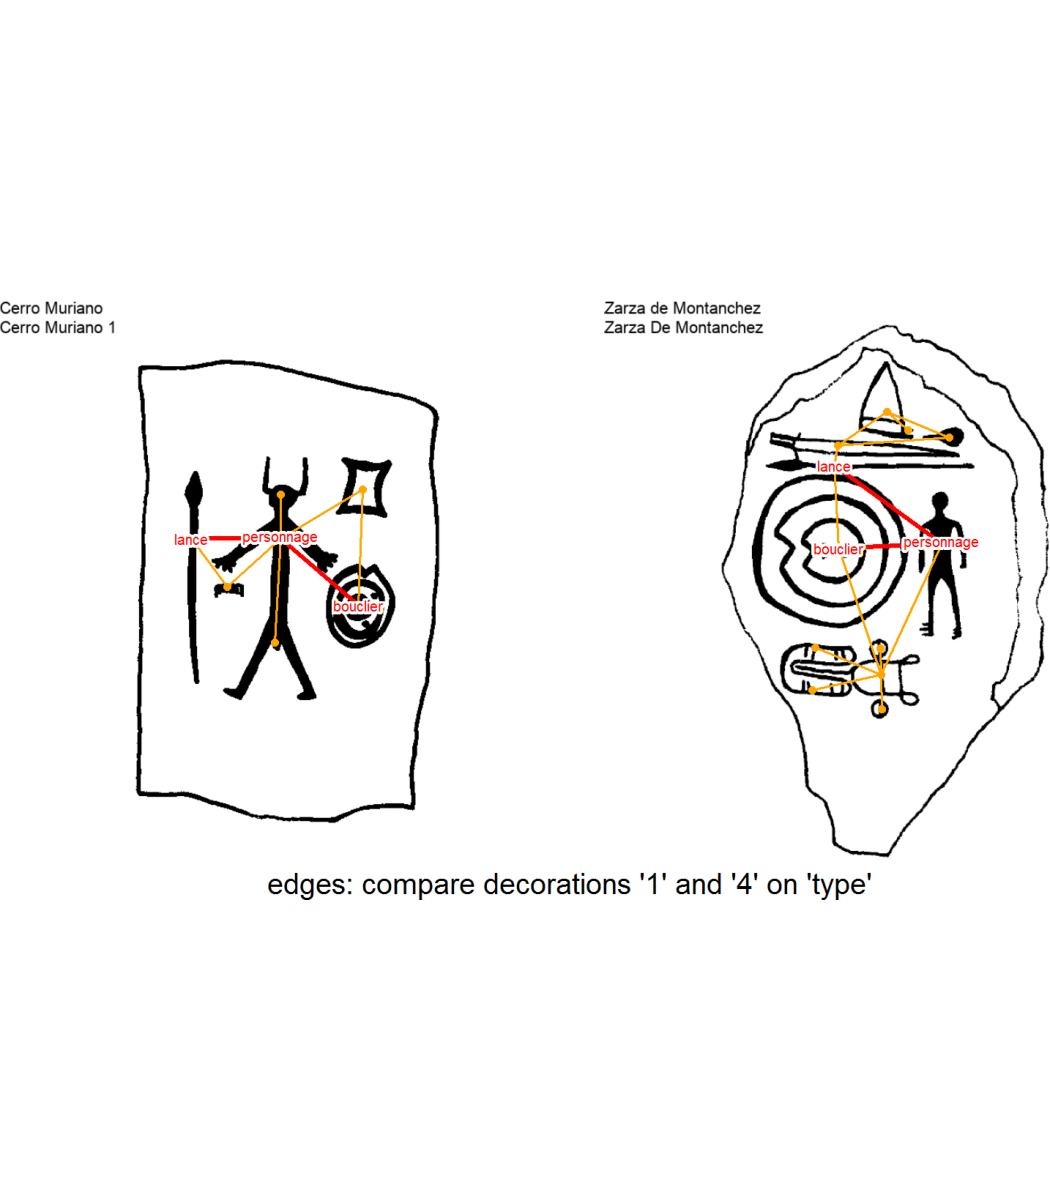
\includegraphics[width=\maxwidth]{figure/unnamed-chunk-12-1} 

}

\caption{\label{fig:figs}comparisons between 1 (Cerro Muriano 1) and 4 (Zarza de Montsanchez) decorations}\label{fig:unnamed-chunk-12}
\end{figure}



The comparison shows that \code{1} (\emph{Cerro Muriano 1}) and \code{4} (\emph{Zarza de Montsanchez}) decorations have two (2) common edges: \code{lance -=- personnage} and \code{personnage -=- bouclier}.

\begin{itemize}
\setlength\itemsep{.1em}
  \item \code{same_nds()} and \code{same_eds()} functions allow to repectively count matching nodes and matching edges between decoration pairwises
\end{itemize}

\code{same_nds()} and \code{same_eds()} allow to repectively count matching nodes and matching edges between decoration pairwises. The result is a square matrix between all pairwise comparisons with the number of common nodes or edges in the cells. For example, we can compute the matrix of common edges.

\begin{kframe}
\begin{verbatim}
R> df.same_edges <- same_eds(lgrph,"type")
R> caption <- "Number of same edges between all decoration pairwise comparisons"
R> print(xtable::xtable(df.same_edges,
+                       caption = caption,
+                       label = "Test_table_2",
+                       size = 8,
+                       digits = c(0)),
+        table.placement="H",
+        include.rownames = TRUE)
\end{verbatim}
\end{kframe}% latex table generated in R 3.6.1 by xtable 1.8-4 package
% Tue Nov 03 09:11:09 2020
\begin{table}[H]
\centering
\begin{tabular}{rrrrr}
  \hline
 & 1 & 2 & 3 & 4 \\ 
  \hline
1 & 0 & 0 & 1 & 2 \\ 
  2 & 0 & 0 & 3 & 7 \\ 
  3 & 1 & 3 & 0 & 1 \\ 
  4 & 2 & 7 & 1 & 0 \\ 
   \hline
\end{tabular}
\caption{Number of same edges between all decoration pairwise comparisons} 
\label{Test_table_2}
\end{table}


For these two last exemples, the edges comparisons between the decoration \code{1} and the decoration \code{4} show that they have two (2) common edges.

\section{Illustrations} \label{sec:illustrations}

As said, since the precise location of the GUs is usualy not registred, the most commonly used method in statistical analysis on prehistorical iconography is the presence of common nodes. In order to demonstrate the first insight of a graph-based analysis of the decorations, we will compare two classifications, the first one based on the "classic" presence of common nodes, the second one based on the presence of common edges.

\begin{table}[H]
\begin{minipage}{.45\textwidth}
\centering
% latex table generated in R 3.6.1 by xtable 1.8-4 package
% Tue Nov 03 09:11:09 2020
\begin{tabular}{rrrrr}
  & 1 & 2 & 3 & 4 \\ 
 1 & 0 & 2 & 3 & 4 \\ 
  2 & 2 & 0 & 5 & 7 \\ 
  3 & 3 & 5 & 0 & 4 \\ 
  4 & 4 & 7 & 4 & 0 \\ 
  \end{tabular}

\captionof{table}{Common nodes table}
\end{minipage}
\begin{minipage}{.45\textwidth}
\centering
% latex table generated in R 3.6.1 by xtable 1.8-4 package
% Tue Nov 03 09:11:09 2020
\begin{tabular}{rrrrr}
  & 1 & 2 & 3 & 4 \\ 
 1 & 0 & 0 & 1 & 2 \\ 
  2 & 0 & 0 & 3 & 7 \\ 
  3 & 1 & 3 & 0 & 1 \\ 
  4 & 2 & 7 & 1 & 0 \\ 
  \end{tabular}

\captionof{table}{Common edges table}
\end{minipage}
\end{table}

Once the heatmap matrices calculated, the native \code{dist()} and \code{hclust()} functions \citep{R19} are calculated from the inverse matrices with the function \code{inv()} of the \pkg{matlib} package \citep{Friendly20}

\begin{figure}[H]
\begin{kframe}
\begin{verbatim}
R> library("matlib")
R> par(mfrow=c(1,2))
R> dist.nodes  <- dist(inv(as.matrix(df.same_nodes)))
R> dist.edges  <- dist(inv(as.matrix(df.same_edges)))
R> plot(hclust(dist.nodes), hang = -1, main = "common nodes")
R> plot(hclust(dist.edges), hang = -1, main = "common edges")
\end{verbatim}
\end{kframe}
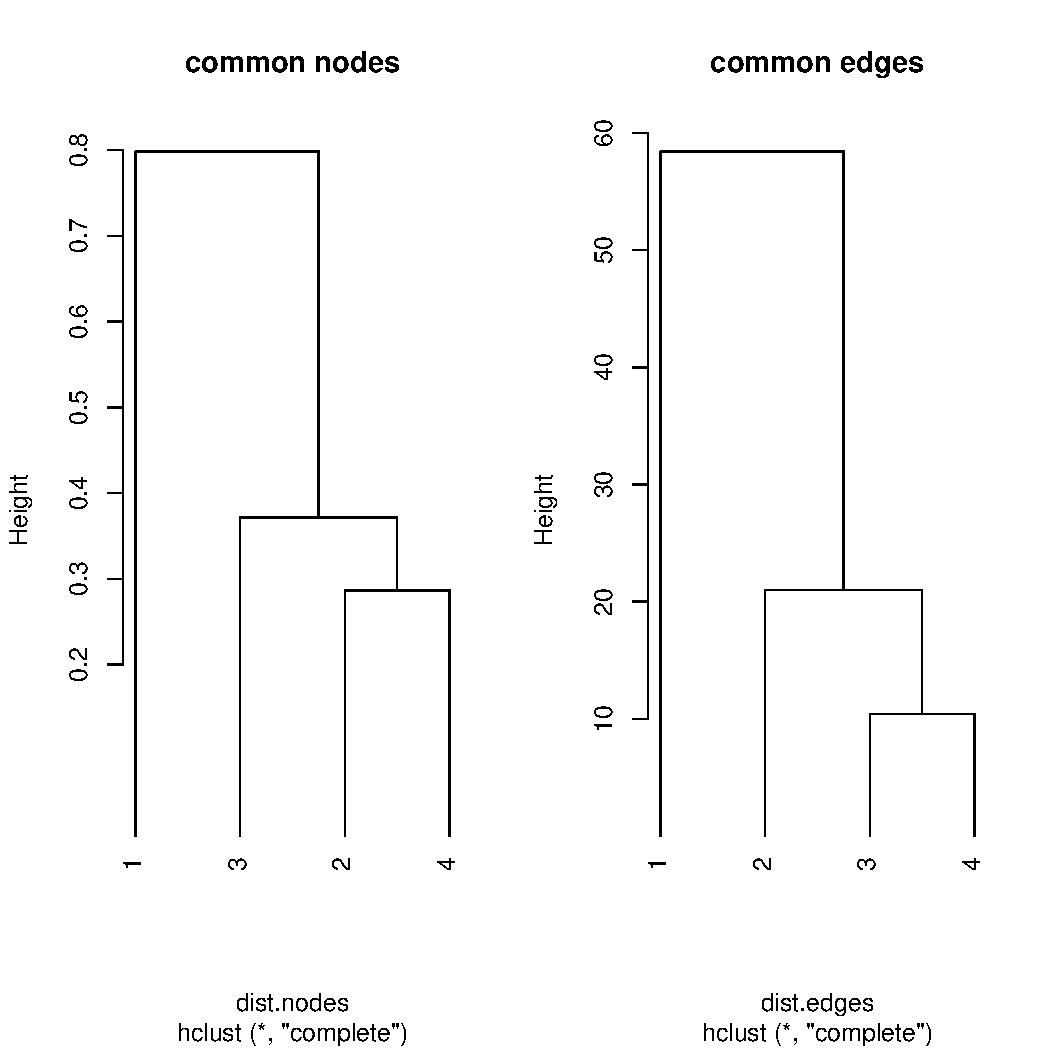
\includegraphics[width=\maxwidth]{figure/unnamed-chunk-16-1} 

\end{figure}

Results of classifications show that for both common nodes and common edges, the most different decorations are \code{1} and \code{4}. These two decorations share four (4) common nodes and, as previously seen, only two (2) common edges.
In any cases decorations \code{2} and \code{3} are closer to decoration \code{4} than to decoration \code{1}, but their classifications changes depending on counting of common nodes or common edges. While decorations \code{2} and \code{4} have 7 common edges and 7 common nodes, plotting the comparisons for for \code{3} and \code{4}, helps to understand the differences between the two classifications.

\begin{kframe}
\begin{verbatim}
R> par(mar=c(0,0,0,0))
R> par(mfrow=c(2,1))
R> g.compar <- list_nds_compar(lgrph,"type")
R> nds_compar.3.4 <- plot_nds_compar(g.compar, c(3,4),
+                                    doss = system.file("extdata", package = "decorr"))
R> plot(image_read(nds_compar.3.4))
R> g.compar <- list_eds_compar(lgrph,"type")
R> eds_compar.3.4 <- plot_eds_compar(g.compar, c(3,4),
+                                doss = system.file("extdata", package = "decorr"))
R> plot(image_read(eds_compar.3.4))
\end{verbatim}
\end{kframe}\begin{figure}[H]

{\centering 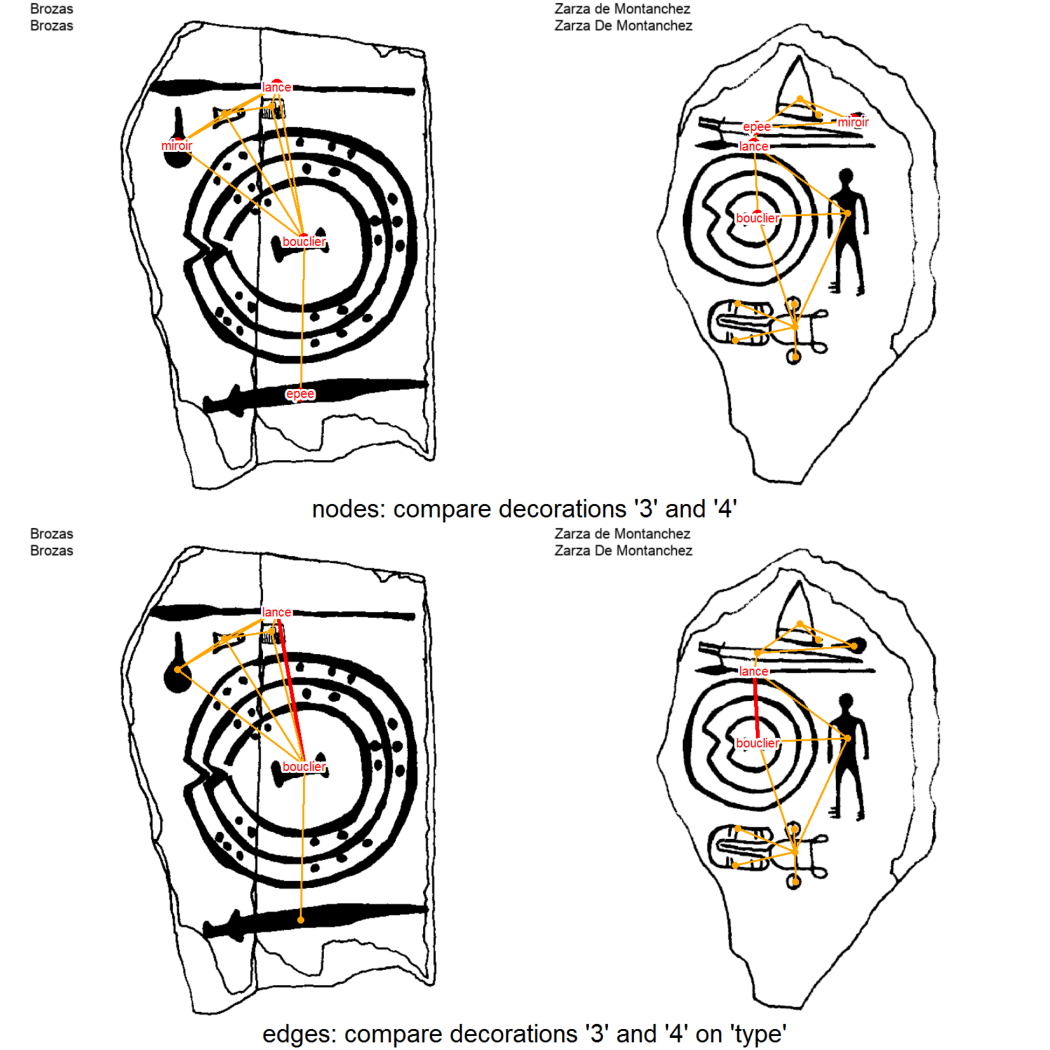
\includegraphics[width=\maxwidth]{figure/unnamed-chunk-17-1} 

}

\caption{\label{fig:figs}Decoration comparisons between 3 and 4}\label{fig:unnamed-chunk-17}
\end{figure}



Decorations \code{3} and \code{4} share four (4) common GUs (\code{bouclier, epee, lance, miroir}) but  these GUs have different spatial organisations with only one common edge (\code{bouclier -=- lance}). At the opposite, decorations \code{2} and \code{4} show more properly the same compositions.

%% -- Summary/conclusions/discussion -------------------------------------------

\section{Summary and discussion} \label{sec:summary}

In this example we propose the iconographical \code{nodes$type} (character, weapon, etc.) GUs as the studied variable, but the user of the package can create and choose any other study variable: color for a painting, technique of realisation, size, etc.
\code{edges$type} can also be extended to other types than normal, attribute, overlapping.
The background is considered as homogeneous but a crack, a pit, a something can also be considered
The plasticity of Graph Theory allows to develop conventions in order to quote the different types of relations s.
Its geographical equivalent is a Thiessen polygon

\begin{table}[H]
% \begin{center}
  \centering
 \begin{tabular}{|p{.5cm} p{.5cm} p{.5cm} p{2cm} p{2cm} p{5cm}|}
 \hline
  % node A & type of edge & node B & undirected & birel & stratigraphical meaning \\
 node 1 & edge type & node 2 & (un)directed & \emph{birel} & description \\
 \hline
  \code{A} & \code{=} & \code{B} & undirected & $ A \cap B = \emptyset $ & \code{A} and \code{B} are disjoint, \code{A} and \code{B} can be contemporaneous \\
  \code{A} & \code{+} & \code{B} & directed & $ A \cap B = A $ & \code{A} and \code{B} are contemporaneous, \code{B} is an attribute of \code{A} \\
  \code{A} & \code{>} & \code{B} & directed & $ A \cap B = \exists $ & \code{A} overlaps \code{B}, \code{A} can be more recent than \code{B} \\
 % \code{1} & = & 2 & undirected & A \cap B = \varnothing & 1 and 2 can be contemporaneous \\
 \hline
\end{tabular}
\caption{Synthesis for the different types of relations between GUs}\label{tab1}
% \end{center}
\end{table}


\begin{leftbar}
As usual \dots
\end{leftbar}


%% -- Optional special unnumbered sections -------------------------------------

\section*{Computational details}

\begin{leftbar}
If necessary or useful, information about certain computational details
such as version numbers, operating systems, or compilers could be included
in an unnumbered section. Also, auxiliary packages (say, for visualizations,
maps, tables, \dots) that are not cited in the main text can be credited here.
\end{leftbar}

The results in this paper were obtained using
\proglang{R}~3.4.1 with the
\pkg{MASS}~7.3.47 package. \proglang{R} itself
and all packages used are available from the Comprehensive
\proglang{R} Archive Network (CRAN) at
\url{https://CRAN.R-project.org/}.


\section*{Acknowledgments}

\begin{leftbar}
All acknowledgments (note the AE spelling) should be collected in this
unnumbered section before the references. It may contain the usual information
about funding and feedback from colleagues/reviewers/etc. Furthermore,
information such as relative contributions of the authors may be added here
(if any).
\end{leftbar}


%% -- Bibliography -------------------------------------------------------------
%% - References need to be provided in a .bib BibTeX database.
%% - All references should be made with \cite, \citet, \citep, \citealp etc.
%%   (and never hard-coded). See the FAQ for details.
%% - JSS-specific markup (\proglang, \pkg, \code) should be used in the .bib.
%% - Titles in the .bib should be in title case.
%% - DOIs should be included where available.

\bibliography{D:/DocumentationArcheo/biblio10}


%% -- Appendix (if any) --------------------------------------------------------
%% - After the bibliography with page break.
%% - With proper section titles and _not_ just "Appendix".

\newpage

\begin{appendix}

\section{More technical details} \label{app:technical}

\begin{leftbar}
Appendices can be included after the bibliography (with a page break). Each
section within the appendix should have a proper section title (rather than
just \emph{Appendix}).

For more technical style details, please check out JSS's style FAQ at
\url{https://www.jstatsoft.org/pages/view/style#frequently-asked-questions}
which includes the following topics:
\begin{itemize}
  \item Title vs.\ sentence case.
  \item Graphics formatting.
  \item Naming conventions.
  \item Turning JSS manuscripts into \proglang{R} package vignettes.
  \item Trouble shooting.
  \item Many other potentially helpful details\dots
\end{itemize}
\end{leftbar}


\section[Using BibTeX]{Using \textsc{Bib}{\TeX}} \label{app:bibtex}

\begin{leftbar}
References need to be provided in a \textsc{Bib}{\TeX} file (\code{.bib}). All
references should be made with \verb|\cite|, \verb|\citet|, \verb|\citep|,
\verb|\citealp| etc.\ (and never hard-coded). This commands yield different
formats of author-year citations and allow to include additional details (e.g.,
pages, chapters, \dots) in brackets. In case you are not familiar with these
commands see the JSS style FAQ for details.

Cleaning up \textsc{Bib}{\TeX} files is a somewhat tedious task -- especially
when acquiring the entries automatically from mixed online sources. However,
it is important that informations are complete and presented in a consistent
style to avoid confusions. JSS requires the following format.
\begin{itemize}
  \item JSS-specific markup (\verb|\proglang|, \verb|\pkg|, \verb|\code|) should
    be used in the references.
  \item Titles should be in title case.
  \item Journal titles should not be abbreviated and in title case.
  \item DOIs should be included where available.
  \item Software should be properly cited as well. For \proglang{R} packages
    \code{citation("pkgname")} typically provides a good starting point.
\end{itemize}
\end{leftbar}

\end{appendix}

%% -----------------------------------------------------------------------------


\end{document}
